\documentclass[journal]{IEEEtran}
% arXiv / IEEE journal version of the AegisRAG paper. Build: latexmk -pdf main.tex (figures in figures/).
\usepackage[T1]{fontenc}
\usepackage{amsmath,amssymb}
\usepackage{graphicx}
\usepackage{booktabs}
\usepackage{url}
\usepackage[hidelinks]{hyperref}
\graphicspath{{figures/}}
\newcommand{\KL}{\mathrm{KL}}

\begin{document}

\title{Reading the Poison: Relative-Entropy Detection of Word-Substitution Poisoning in a Cybersecurity RAG Knowledge Base}

% Co-authorship to be agreed with Dr Nikos Komninos before submission.
\author{Ali~Yousefi%
\thanks{A.~Yousefi is with the Department of Computer Science, City St George's, University of London, London, UK.}}

\markboth{Preprint, 2026}{Yousefi: Relative-Entropy Detection of Word-Substitution Poisoning in RAG}

\maketitle

\begin{abstract}
Retrieval-augmented generation (RAG) makes the knowledge base part of a system's trust boundary. We study word-substitution poisoning, in which an attacker rewrites existing passages with plausible synonyms (PWWS, TextFooler) instead of injecting new text, on a cybersecurity RAG system built from MITRE ATT\&CK and CAPEC, with a reviewed benchmark, paired repeated runs and a formatting-only control. Poisoning lowers answer correctness from 0.714 to 0.555, entirely on questions whose source was perturbed, mainly by displacing evidence and causing refusals rather than by injecting misinformation. Treating detection as a relative-entropy problem, whole-distribution divergences fail (letter-frequency KL AUROC 0.33, Jensen--Shannon 0.47), but a per-word log-ratio between a word and its most probable synonym works, and a language-model reference raises AUROC from 0.82 to 0.95 while staying at chance on the control. It clearly outperforms whole-passage perplexity (0.77), matches a windowed perplexity filter, and additionally names the word it suspects was replaced. As a retrieval filter it halves the poisoned text reaching the generator and removes confidently wrong answers at no measurable cost on clean data, but it does not restore correctness. An adaptive attacker that matches word frequencies evades a frequency reference but not the language-model one, and an attacker that must also keep passages as probable under the language model succeeds on none of 57 sections. Both findings transfer to TextFooler in live runs, whereas an answer-level evidence check misses the incomplete answers this attack causes. All records, code and analyses are released.
\end{abstract}

\begin{IEEEkeywords}
Retrieval-augmented generation, data poisoning, adversarial text, relative entropy, large language models, adaptive attacks.
\end{IEEEkeywords}

\section{Introduction}
\IEEEPARstart{A}{} RAG system answers a question by retrieving passages from a knowledge base and asking a language model to answer from them~\cite{lewis2020rag}. Its answers are therefore only as trustworthy as the passages it reads. Knowledge-corruption attacks show that a handful of injected passages can steer answers to attacker-chosen targets~\cite{zou2025poisonedrag,zhong2023poisoning}. A less visible threat is \emph{editing} existing passages: word-level adversarial attacks such as PWWS~\cite{ren2019pwws} and TextFooler~\cite{jin2020textfooler} replace words with synonyms until a classifier changes its decision, leaving text that still reads almost normally. Such perturbations have been shown to degrade an LLM-based threat-detection framework through its knowledge base~\cite{ikbarieh2025rag}.

We ask three questions about this threat in a cybersecurity question-answering setting: (i) how much word-substitution poisoning hurts a RAG system, and through what mechanism; (ii) whether an information-theoretic detector can find the poisoned passages, and which reference distribution makes it work; and (iii) whether the detector survives an attacker who knows it, and what evasion costs the attacker.

We approach detection through relative entropy. If a passage's word distribution $p$ is compared with a reference $q$ of normal text, $\KL(p\,\|\,q)=\sum_x p(x)\log_2 \frac{p(x)}{q(x)}$~\cite{kullback1951} should rise when words are swapped for unusual synonyms. We show that the full sum is the wrong tool and that one of its terms, the log-ratio between a word and its likely original under $q$, is the right one, provided $q$ is good enough. This adapts frequency-guided substitution detection~\cite{mozes2021fgws} to a domain reference and then to a language-model reference.

\textbf{Contributions.}
\begin{itemize}
\item A controlled, fully recorded testbed: clean, PWWS-poisoned and formatting-only control knowledge bases; a reviewed benchmark with source anchors; paired runs with create-only, checksummed records (Section~\ref{sec:testbed}).
\item A measured mechanism: substitution poisoning works mainly by \emph{displacing} evidence and causing abstention, and only rarely by misinformation the model repeats (Section~\ref{sec:mechanism}).
\item A family of relative-entropy detectors evaluated against a formatting-only control and against perplexity filters, showing that whole-distribution measures fail and that \emph{local} language-model improbability works, with the synonym gap as an explainable member of that family (Section~\ref{sec:detection}).
\item Live evaluations of three retrieval-time defences and an answer-level evidence check, showing a consistent safety/utility trade-off (Sections~\ref{sec:defences} and~\ref{sec:evidence}).
\item Adaptive attackers at increasing knowledge and budget, with a swap-level explanation of why fooling the classifier while staying probable under a language model is hard, and a second attack to test generality (Sections~\ref{sec:adaptive} and~\ref{sec:textfooler}).
\end{itemize}

\section{Related Work}
\textbf{Poisoning RAG.} PoisonedRAG~\cite{zou2025poisonedrag} injects passages that are both retrieved and induce a target answer; Zhong et~al.~\cite{zhong2023poisoning} craft passages retrieved for many queries. Both \emph{add} text. Ikbarieh et~al.~\cite{ikbarieh2025rag} perturb an existing knowledge base with TextFooler and show degraded threat detection. We study in-place substitution and measure where along retrieval and generation the damage occurs.

\textbf{Word-substitution attacks and their detection.} PWWS~\cite{ren2019pwws} ranks words by saliency and replaces each with the WordNet~\cite{miller1995wordnet} synonym that most reduces the classifier's confidence; TextFooler~\cite{jin2020textfooler} draws substitutes from counter-fitted embeddings; both are implemented in TextAttack~\cite{morris2020textattack}. FGWS~\cite{mozes2021fgws} detects such examples by replacing infrequent words with frequent synonyms and measuring the change in the classifier's output. Our synonym gap keeps FGWS's observation that adversarial substitutes are often rarer than the words they replace, but scores the text against a reference distribution without access to the attacked classifier, so it can run at retrieval time.

\textbf{Perplexity filters.} Language-model perplexity is a standard model-agnostic filter for adversarial text: adversarial suffixes have very high perplexity~\cite{alon2023perplexity}, and windowed perplexity filters are an effective baseline against them~\cite{jain2023baseline}. RAGuard~\cite{cheng2025raguard} applies chunk-wise perplexity and similarity filtering to RAG poisoning. We compare against whole-passage and windowed perplexity computed with the same language model as our detector.

\textbf{Defending RAG.} RobustRAG~\cite{xiang2024robustrag} isolates and aggregates per-passage answers with certifiable guarantees; TrustRAG~\cite{zhou2025trustrag} clusters retrieved passages to identify suspicious groups; Corrective RAG~\cite{yan2024crag} grades retrieval quality and falls back to other sources. Evidence-support checks such as RAGAS faithfulness~\cite{es2024ragas} assess whether an answer follows from its sources, and sampling-based checks~\cite{manakul2023selfcheckgpt} target hallucination. These defences mostly target injected passages or answer quality; we evaluate passage-level filtering of \emph{edited} text, which needs no change to generation.

\section{Threat Model and Testbed}\label{sec:testbed}
\textbf{System.} A FastAPI backend retrieves the top~3 passages from Qdrant (all-MiniLM-L6-v2 embeddings; 500-character chunks with 100 overlap) and answers with gpt-4o-mini at temperature~0 under a fixed prompt that requires answering only from the context. A web interface shows clean and poisoned answers side by side, with each defence as a selectable mode.

\textbf{Knowledge base.} 18 documents of MITRE ATT\&CK and CAPEC material covering 14 attack types in 5 categories (DDoS, injection, malware, reconnaissance, spoofing), split into 200 passages.

\textbf{Attacker.} The attacker can edit eligible text in the knowledge base but not the questions, retrieval or generation settings, or the evaluation. PWWS (TextAttack) attacks a DistilBERT attack-type classifier trained on the same material, used as a \emph{surrogate}: a section is rewritten when PWWS flips the surrogate's label. Of 88 eligible sections, 31 are already misclassified and skipped; PWWS succeeds on 38 of the remaining 57 (a retrained surrogate, used for all adaptive experiments and their matched control, gives 39). Original and adversarial text are recorded in an attack manifest.

\textbf{Formatting-only control.} The poisoning script also flattens the layout of the sections it rewrites. A control corpus applies the same flattening to the same sections with the original words. Retrieval on the control equals clean, so layout alone does not cause the damage.

\textbf{Benchmark and protocol.} 44 reviewed questions, each with atomic reference facts and an exact source anchor; development and held-out questions are separated by source document (35/9). Every question runs 3~times per condition, paired by schedule index with alternated condition order. Correctness (against reference facts) and faithfulness (against retrieved passages) are scored by an LLM judge~\cite{zheng2023judge} with a fixed rubric; retrieval relevance by Hit@3 under a section-level rule; \emph{edited-text exposure} records whether any attacker-edited word reached the generator. Retrieval is deterministic across repetitions, so the question is the unit of analysis: we report question-level cluster-bootstrap 95\% intervals (10{,}000 resamples) and two-sided Wilcoxon signed-rank tests. Every run writes create-only JSON records with a SHA-256 completion manifest, and a script checks every headline number in this paper against its source file.

\section{Relative-Entropy Detectors}\label{sec:detectors}
Let a passage contain words $w_1,\dots,w_n$ with empirical distribution $p$, and let $q$ be a reference distribution.

\textbf{Whole-passage divergences.} $\KL(p\,\|\,q)$~\cite{kullback1951}, Jensen--Shannon divergence~\cite{lin1991js} and mean surprisal $-\frac{1}{n}\sum_i \log_2 q(w_i)$; we also report KL over letter frequencies, the textbook illustration of relative entropy.

\textbf{Synonym gap.} For each content word $w$ with WordNet synonyms $S(w)$,
\begin{equation}
g(w)=\max_{s\in S(w)}\big[\log_2 q(s)-\log_2 q(w)\big],
\end{equation}
the number of bits by which the most probable synonym beats the word actually used. This is the log-ratio term of KL evaluated at the substitution itself: the PWWS substitute ``abnegate'' scores high because its likely original ``deny'' is far more probable. A passage's score is the mean of its three largest gaps.

\textbf{References.} (i)~General English word frequencies; (ii)~a \emph{domain} reference: leave-one-document-out counts from the rest of the knowledge base interpolated 50/50 with English, which needs no clean copy of the poisoned document; (iii)~the same with a Dirichlet prior, $q(w)=\frac{c(w)+\mu q_{\mathrm{en}}(w)}{N+\mu}$, $\mu=2000$~\cite{zhai2004smoothing}; (iv)~a \emph{contextual} reference from a small causal language model, distilgpt2~\cite{radford2019gpt2}. For (iv), the candidates are the 10 words with the largest domain gap and, for each, its 5 most probable synonyms $s$:
\begin{equation}
g_{\mathrm{ctx}}(w,s)=\log_2 p_{\mathrm{LM}}(\text{passage}, w\!\to\! s)-\log_2 p_{\mathrm{LM}}(\text{passage}),
\end{equation}
and the passage score is again the mean of the three largest gaps.

\textbf{Perplexity baselines.} With the same language model: \emph{mean surprisal} (log$_2$ perplexity of the whole passage) and \emph{top-5 surprisal}, the mean of the five most surprising tokens, a windowed filter in the spirit of~\cite{jain2023baseline}.

All scores use only information a defender has; attack labels are used for evaluation only. Thresholds are fixed on development documents at a 10\% false-positive rate and never tuned on held-out documents or live answers.

\section{Results}
\subsection{The attack and its mechanism}\label{sec:mechanism}
\begin{table}[t]
\caption{Effect of PWWS poisoning (44 questions, 132 paired answers per condition).}\label{tab:attack}
\centering\footnotesize\setlength{\tabcolsep}{3pt}
\begin{tabular}{@{}lccc@{}}
\toprule
Stratum & Hit@3 & Correctness & $\Delta$ [95\% CI]\\
\midrule
All & .705$\to$.568 & .714$\to$.555 & $-$.159 [$-$.254, $-$.068]\\
Target perturbed (27) & .630$\to$.444 & .682$\to$.432 & $-$.250 [$-$.383, $-$.124]\\
Not perturbed (17) & .824$\to$.765 & .765$\to$.750 & $-$.015 [$-$.083, .069]\\
\bottomrule
\end{tabular}
\end{table}
The degradation is confined to questions whose source section was perturbed (Table~\ref{tab:attack}); questions answered from untouched sections of the same poisoned corpus are unaffected. Together with the formatting-only control, this attributes the effect to the substitutions. The mechanism is mostly \emph{displacement}: abstentions rise from 26 to 45 of 132 answers, and of the 48 answers whose correctness fell by at least 0.25, 27 abstained and 31 had lost the relevant passage from the top~3. Confidently wrong answers rose only from 0 to 2; in both, the model repeated a substituted phrase (``Engraft Malicious Package'', originally ``implants malicious software'') as if it were a named attack stage.

\subsection{Detection}\label{sec:detection}
\begin{table*}[t]
\caption{Detection of passages containing substituted words (AUROC). Brackets: 95\% bootstrap intervals resampling documents. 191 passages (193 for TextFooler); edited passages: 47 PWWS, 59 matched rerun, 82 TextFooler, 13 adaptive. The last row counts edits flagged at the contextual threshold (4.46 bits) frozen on PWWS development documents, which flags 9--14\% of unedited passages.}\label{tab:detect}
\centering\footnotesize\setlength{\tabcolsep}{4pt}
\begin{tabular}{@{}lccccc@{}}
\toprule
Detector & PWWS & PWWS rerun & TextFooler & Control (layout only) & Frequency-matched adaptive\\
\midrule
Letter-frequency KL & 0.33 & -- & 0.28 & 0.35 & 0.36\\
Word KL vs domain & 0.72 & -- & 0.83 & 0.62 & 0.50\\
Jensen--Shannon vs domain & 0.47 & -- & 0.48 & 0.43 & 0.44\\
Mean surprisal (perplexity) & 0.77 & 0.77 & 0.82 & 0.45 & 0.73\\
Top-5 surprisal (windowed perplexity) & 0.91 & 0.93 & 0.92 & 0.56 & 0.85\\
Synonym gap, domain $q$ & 0.82 [.72, .90] & 0.88 [.82, .94] & 0.90 [.85, .94] & 0.67 [.57, .77] & 0.47 [.33, .72]\\
Synonym gap, Dirichlet $q$ & 0.83 & -- & 0.90 & 0.68 & 0.48\\
\textbf{Contextual synonym gap} & \textbf{0.95} [.87, .99] & \textbf{0.97} [.93, 1.0] & \textbf{0.91} [.84, .97] & \textbf{0.53} [.45, .60] & \textbf{0.92} [.54, .96]\\
\midrule
\emph{Edits flagged, frozen contextual threshold} & 42/47 & 54/59 & 70/82 & -- & 10/13\\
\bottomrule
\end{tabular}
\end{table*}

Four findings follow (Table~\ref{tab:detect}, Fig.~\ref{fig:robust}). First, \textbf{whole-distribution measures fail}: letters keep English statistics under word swaps, and KL, JS or perplexity over the whole passage dilute the handful of changed words among about eighty. Second, \textbf{the per-word log-ratio works}, and the choice of $q$ matters more than the divergence or smoothing (Dirichlet vs interpolation: 0.83 vs 0.82). Third, \textbf{the contextual reference is stronger and cleaner}: it improves on the word-frequency gap on both PWWS corpora (paired differences $+0.13$ [$+0.03$, $+0.21$] and $+0.09$ [$+0.03$, $+0.16$]) and is at chance on the control, where the word-frequency gap still scores 0.67 because part of its signal comes from which sections were attacked. Fourth, \textbf{locality is what matters}: the contextual gap beats whole-passage perplexity on PWWS and TextFooler (paired differences $+0.18$ [$+0.11$, $+0.26$] and $+0.10$ [$+0.03$, $+0.16$]) but is statistically indistinguishable from windowed perplexity ($+0.04$ [$-0.003$, $+0.08$] on PWWS, $-0.01$ [$-0.07$, $+0.03$] on TextFooler). What the synonym gap adds over a windowed perplexity filter is an explanation: of 27 edited passages the word-frequency gap flags, 22 name the exact replaced word with its likely original (abnegate$\to$deny, meshing$\to$network), and at frozen thresholds it has a slightly lower false-positive rate on every attacked corpus.

\begin{figure}[t]
\centering
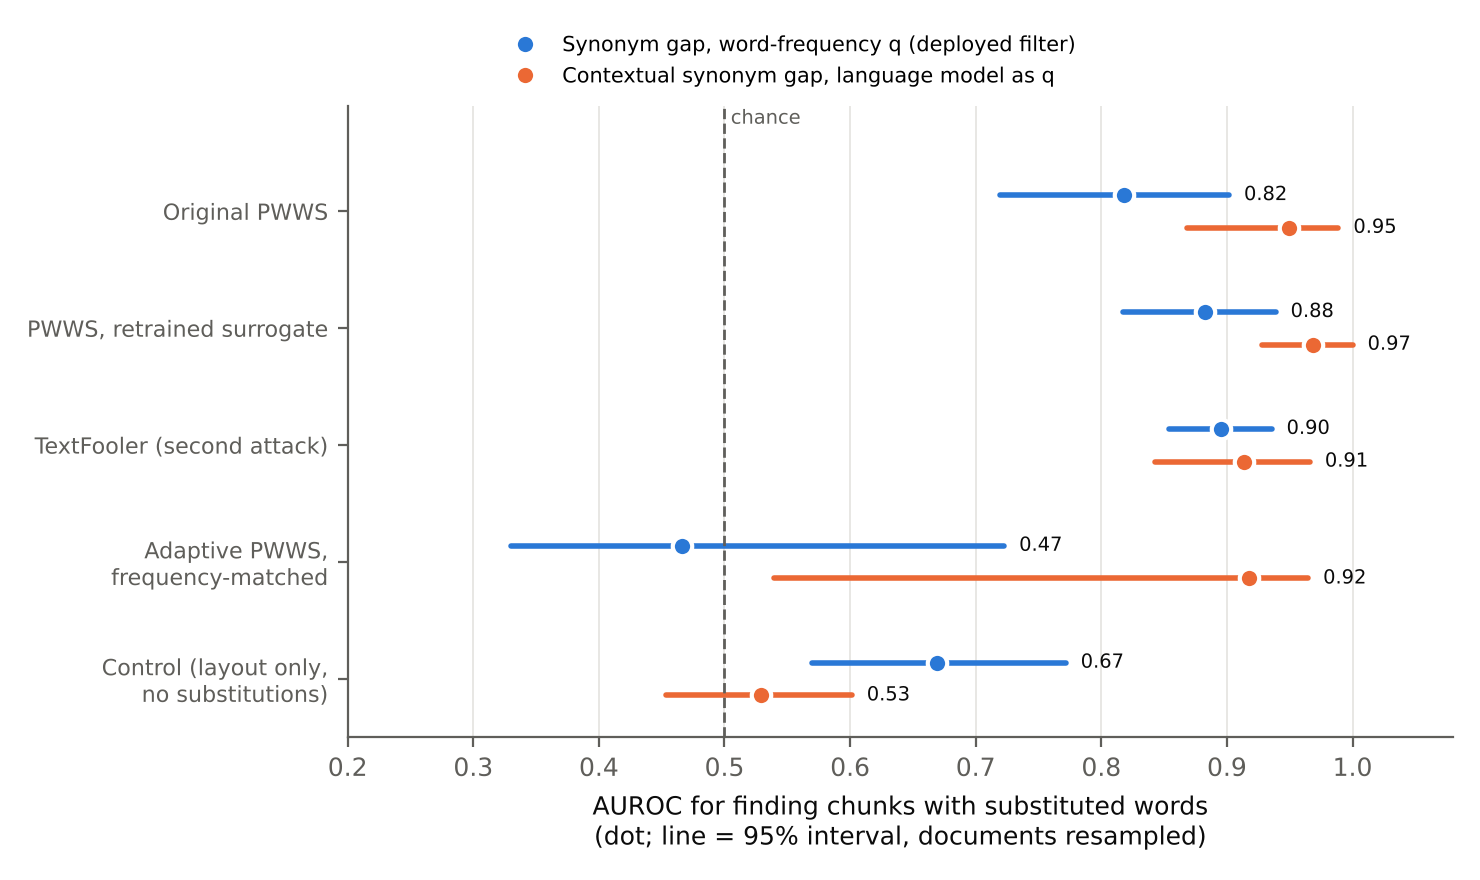
\includegraphics[width=\columnwidth]{fig6_detector_robustness.png}
\caption{Word-frequency versus contextual synonym gap on every corpus, with document-clustered 95\% intervals.}\label{fig:robust}
\end{figure}

\subsection{Live defences}\label{sec:defences}
Each defence retrieves 10 candidates, scores them and passes 3 to the generator: \emph{drop} removes candidates above the word-frequency threshold (7.23 bits); \emph{repair} first replaces words with a gap above 9.5 bits by their likely original and keeps the passage if it then scores under the threshold; \emph{contextual} drops with the contextual gap (4.46 bits). Each was run live on the full benchmark against both corpora (792 records per run).

\begin{table}[t]
\caption{Live defences on the poisoned corpus (44 questions $\times$ 3; $p$: Wilcoxon vs no defence). Clean cost: correctness change on the clean corpus.}\label{tab:defence}
\centering\small
\setlength{\tabcolsep}{3pt}
\begin{tabular}{@{}lccccc@{}}
\toprule
Defence & Exposure & Correct. & Wrong & Abst. & Clean cost\\
\midrule
None & .409 & .555 & 2 & 45 & --\\
Drop (freq.) & .273$^{a}$ & .526 & 0 & 53 & $-$.064\\
Repair & .364 & .506 & 0 & 54 & $-$.042\\
\textbf{Drop (ctx.)} & \textbf{.204}$^{b}$ & .485$^{c}$ & \textbf{0} & 63 & $\mathbf{-.013}$\\
\bottomrule
\multicolumn{6}{@{}l}{\footnotesize $^{a}p=0.031$; $^{b}p=0.012$; $^{c}p=0.020$.}
\end{tabular}
\end{table}

All three defences remove the confidently wrong answers (Table~\ref{tab:defence}). The contextual filter halves the poisoned text that reaches the model and is the cheapest on clean data (it flags 8.4\% of clean candidates against 10.9\% for the word-frequency filter). None restores correctness: when the passage that answers a question is the poisoned one, removing it leaves the model without evidence, and it declines rather than guesses. Repair does not help either, because word-level WordNet repair restores too few substitutions (recall 0.12 at precision 0.89). \textbf{Filtering makes a poisoned knowledge base safe to read; it does not make it useful again.}

\subsection{Adaptive attackers}\label{sec:adaptive}
\begin{table}[t]
\caption{Adaptive attackers (same retrained surrogate and 57 attackable sections; the evasion rule is the only difference). AUROC of the word-frequency and contextual synonym gaps.}\label{tab:adaptive}
\centering\small
\setlength{\tabcolsep}{3pt}
\begin{tabular}{@{}lcccc@{}}
\toprule
Attacker & Sections & Edits & Freq. & Ctx.\\
\midrule
Unrestricted PWWS & 39 & 59 & .88 & .97\\
1st order: frequency-matched & 8 & 13 & \textbf{.47} & \textbf{.92}\\
2nd order, strict & \textbf{0} & 0 & -- & --\\
2nd order, $\le$4.46 bits & \textbf{0} & 0 & -- & --\\
2nd order, $\le$20 bits & \textbf{0} & 0 & -- & --\\
2nd order, $\le$100 bits & 5 & 6 & .51 & .78\\
2nd order, $\le$300 bits & 8 & 13 & .47 & .92\\
\bottomrule
\end{tabular}
\end{table}

A first-order attacker that only swaps to words at least as frequent under the defender's $q$ evades the word-frequency detector completely, as designed, but the contextual detector still finds its edits (Table~\ref{tab:adaptive}): it matched how common its words are, not whether they fit the sentence. Evasion is expensive: success falls from 39 to 8 sections.

A second-order attacker that must also keep each passage at least as probable under the detector's language model succeeds on none. Of the 550 swaps unrestricted PWWS used in its 39 successful attacks, 109 (20\%) satisfy the frequency rule but only 9 (1.6\%) leave the passage at least as probable, and 5 satisfy both; the median swap makes its passage 17.9 bits less probable. Natural source text sits close to a local maximum of language-model likelihood, and the substitutions that move a classifier are, almost by definition, ones that move the text away from it.

Relaxing the rule (Fig.~\ref{fig:budget}), the attacker still succeeds on no section when it may lose up to 4.46 bits, the contextual threshold, or 20 bits. At 100 bits it succeeds on 5 sections, whose 6 edited passages the contextual detector scores at 0.78 (the frozen filter flags 3; the interval is wide). At 300 bits the language-model rule stops binding and the attack reproduces the frequency-matched knowledge base exactly, whose edits the contextual filter flags 10 of 13. In this attacker family, no attacker evades the contextual detector: those that satisfy its rule fail to attack, and those that succeed are flagged.

\begin{figure}[t]
\centering
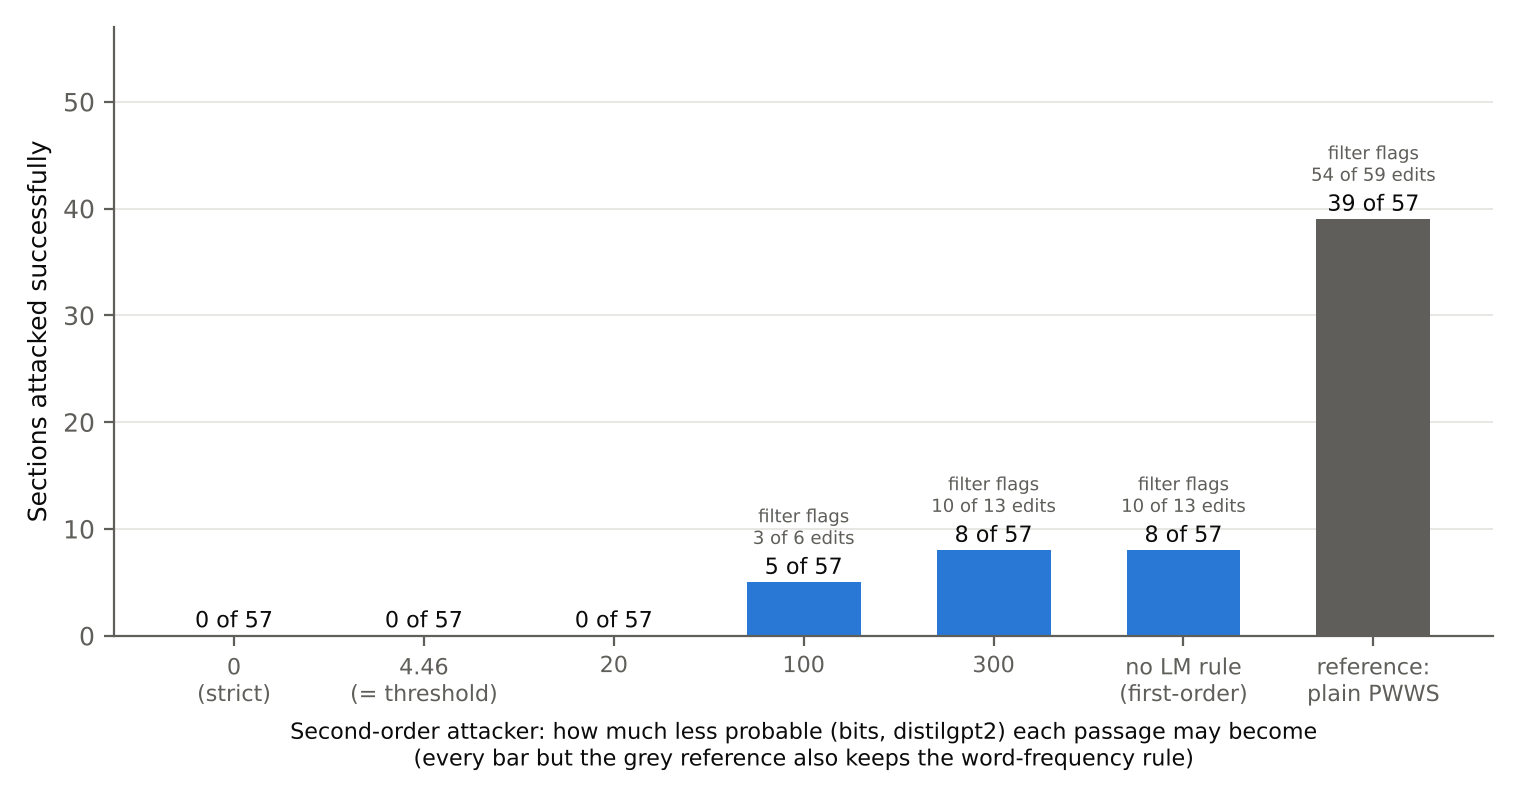
\includegraphics[width=\columnwidth]{fig7_attacker_budget.png}
\caption{Second-order attacker: successful sections as the allowed loss of language-model likelihood grows, with the share of resulting edits flagged by the frozen contextual filter.}\label{fig:budget}
\end{figure}

\subsection{A second attack}\label{sec:textfooler}
TextFooler draws substitutes from word embeddings rather than WordNet. With the same surrogate and sections it is the stronger attack: 49 of 57 sections and 82 edited passages. Both synonym-gap detectors transfer without change (Table~\ref{tab:detect}); at thresholds frozen on PWWS development documents the contextual filter flags 70 of 82 edits (85\%) at a 9\% false-positive rate, against 43 of 82 for the word-frequency filter.

Run live with the same frozen thresholds, TextFooler is also the more pervasive attack: edited text reaches the generator on 82\% of questions (PWWS: 41\%), and correctness falls from 0.714 to 0.564 ($p=0.002$), again through refusals rather than confident errors. The word-frequency filter barely changes exposure (82\%$\to$80\%): when most candidates are edited, dropping some mostly promotes others. The contextual filter cuts exposure to 52\% ($p<0.001$; versus the word-frequency filter, $p=0.003$), with the same cost as on PWWS: correctness falls further (0.447) and refusals rise from 54 to 74 of 132.

\subsection{Checking answers instead of passages}\label{sec:evidence}
We also evaluated an answer-level indicator: a separate verifier call splits each drafted answer into claims, judges each against the retrieved passages, and must quote its evidence verbatim (checked in code); the answer is withheld unless every claim is supported. Replayed on 352 recorded answers (one repetition of all questions in eight conditions), it is not a useful error detector here. Of the 238 answers that are not refusals, 38\% are not fully correct, but only 28\% of flagged answers are (precision 0.28 [0.13, 0.48]); it flags 20\% of errors and 31\% of correct answers. Substitution poisoning mostly removes evidence, so the typical error is an incomplete answer whose every statement is grounded (68 of 89 partial answers pass). It did withhold the one confidently wrong answer. Against in-place substitution, the defence has to act on passages before generation; checking grounding afterwards cannot see what is missing.

\section{Discussion}
\textbf{Why the log-ratio and not the sum.} $\KL(p\,\|\,q)$ is a sum of log-ratio terms weighted by $p$. Substitution changes a handful of terms whose weight is small and swamped by the passage's topic, which also differs from $q$. The synonym gap evaluates the log-ratio only where the attack acts, comparing each word with the alternative the attacker would have replaced.

\textbf{Why a better $q$ beats a better divergence.} Smoothing and symmetry leave the result unchanged, while moving from a unigram to a contextual $q$ changes it substantially: a unigram reference can only say a word is rare, a contextual one says it is unlikely \emph{here}. The perplexity baselines point the same way: what matters is evaluating improbability locally, where the edit is; the synonym gap does so while naming the suspected original.

\textbf{Detection is not restoration.} In this corpus the passage that answers a perturbed question is usually the perturbed one, so any filter that removes poison also removes evidence. Restoring utility requires restoring the original text, for example from a trusted structured source or a masked language model conditioned on the domain.

\textbf{Detection constrains the attacker.} Each additional constraint needed to evade a better reference removes most of the swaps that make the attack work; against the contextual detector the strict attacker has no successful attack in our setting.

\section{Limitations}
One knowledge base (18 documents), one generation model, one embedding model and 44 questions, of which 9 are held out; the adaptive results rest on 13 and 6 edited passages. The second-order attacker constrains whole-passage likelihood but does not optimise against the detector's score directly; such an attacker, a masked-language-model attack, or a larger reference model may behave differently. The attack targets a surrogate classifier, not the RAG pipeline itself; transfer to retrieval and answers is measured, not optimised. Correctness is scored by an LLM judge; a blind manual check of 75 stratified answers is in progress. Thresholds were fixed once on development data, and the safety/utility balance depends on them.

\section{Ethics}
The attacks edit a local copy of public MITRE material; no system is attacked and no malware is executed. No personal data is used; question and passage text is sent to a commercial LLM API. Detection scores are evidence for review, not proof that a passage is clean or an answer true.

\section{Reproducibility}
Code, corpora, attack manifests, run records (create-only JSON with SHA-256 completion manifests) and analysis scripts are released with the paper. A verification script recomputes every headline number from saved files and re-hashes all run records.

\section*{Acknowledgment}
The relative-entropy framing was suggested by Dr Nikos Komninos. AI tools assisted with coding, analysis and drafting; the author checked all code, numbers and references and takes full responsibility for the content.

\bibliographystyle{IEEEtran}
\bibliography{refs}

\end{document}
